\section{Introduction}
Existing test-time adaptation methods often fail when deployment shifts across streams, backbones, or tasks. In TTA, a source-trained model updates itself from unlabeled target inputs at inference. This source-free setting is used for corruptions, covariate shift, natural shifts, dense prediction, and prompt-only VLM adaptation~\citep{schneider2020covariateshift,wang2021tent,niu2022eata,wang2022cotta,niu2023sar,yuan2023rotta,lee2024deyo,karmanov2024tda,farina2024zero,niu2024foa,dai2025freetta,sheng2025ttavlm,ma2025adadem,duan2025lifelong,ma2025surgeon,tan2025eatac}. Its central problem is reliability: weak target evidence can corrupt the next model state.

Recent methods use confidence filters, regularization, teachers, memories, gradient constraints, or prompt tuning, and usually instantiate these safeguards for a particular model or task interface. Our experiments expose corresponding changes in failure behavior: a filter that works for reset corruption evaluation can fail under a non-i.i.d. stream, and image-level loss scaling does not directly specify how dense pixels or prompt views should contribute. We therefore study a reliability decomposition with three linked operations: \core{} selects corroborated evidence, \care{} anchors accepted updates against drift, and \sane{} normalizes the update by selected entities. ATLAS instantiates this decomposition separately for each evaluated interface; it does not assume that the trainable parameters, gates, optimizer, or numerical settings are identical across tasks.

\begin{wrapfigure}{r}{0.48\textwidth}
\vspace{-10pt}
\centering
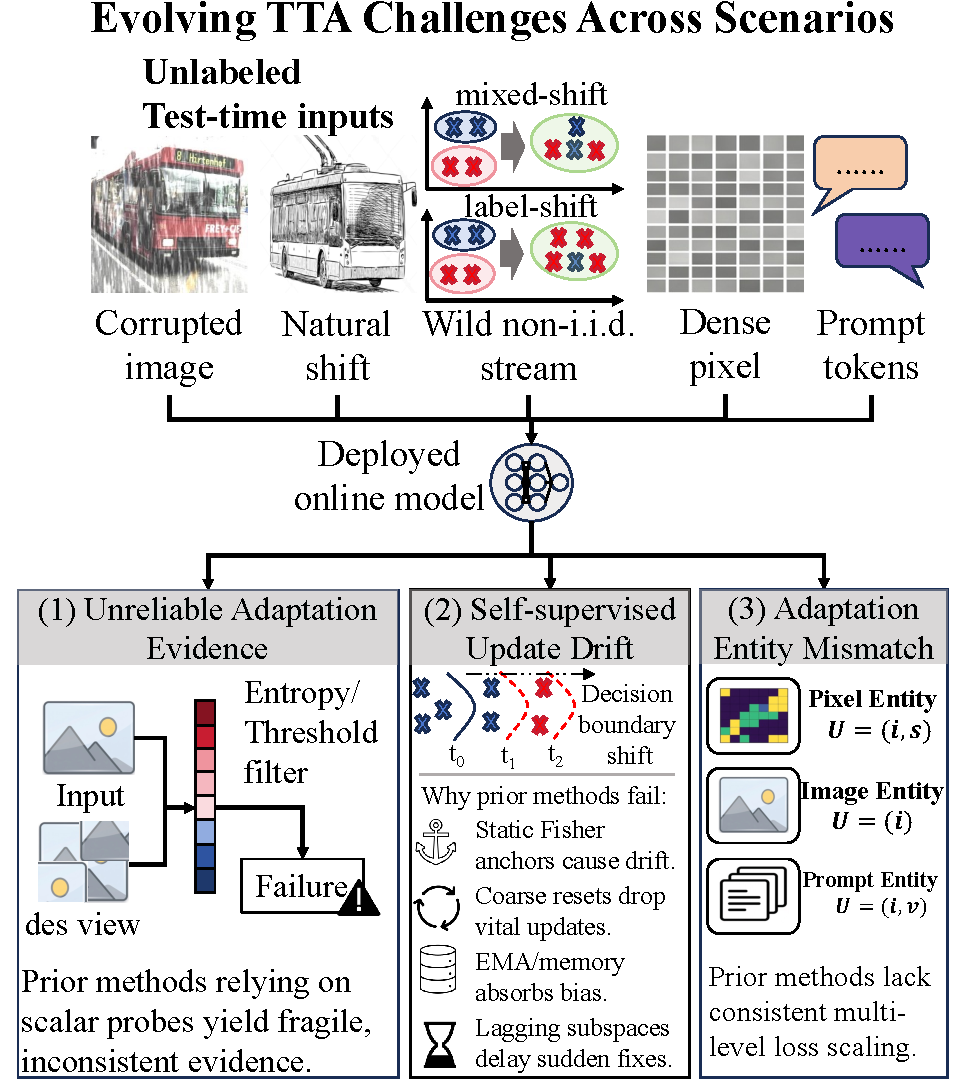
\includegraphics[width=\linewidth]{figures/fig1.pdf}
\caption{Overview of evolving test-time adaptation (TTA) challenges.}
\label{fig:tta_challenges}
\vspace{-10pt}
\end{wrapfigure}


The first problem is \emph{unreliable adaptation evidence}. \textsc{Tent} uses entropy as the adaptation signal, and later methods add filters, redundancy control, instability checks, or destructive probes~\citep{wang2021tent,niu2022eata,niu2023sar,lee2024deyo}. Low entropy alone, however, does not establish that a prediction is correct, and multiple target views can agree on the same mistake. Our hypothesis is that an entity is safer to update when semantics-preserving views corroborate the raw and source predictions and a structure-breaking view produces the expected sensitivity. Motivated by reliability analyses and VLM multi-view aggregation~\citep{press2024entropyenigma,farina2024zero}, \core{} operationalizes this hypothesis. We test it through selection ablations, same-role replacements, and signal diagnostics rather than treating confidence as sufficient evidence.

The second problem is \emph{drift after acceptance}. Because an online model supplies its own pseudo-targets, a selected sample can still move later predictions toward an unstable class. Fisher regularization, flat-minima recovery, teacher restoration, memory, gradient projection, and class debiasing provide different forms of drift control~\citep{niu2022eata,niu2023sar,wang2022cotta,yuan2023rotta,duan2025lifelong,ma2025adadem}. We hypothesize that an accepted update should have a stable reference appropriate to its model interface. \care{} uses source-relative clipping where direct source support is informative and class-centered support where online class geometry is the chosen reference. CORE-only and CORE+CARE ablations, together with continual and wild streams, test whether this anchoring reduces accumulated error.

The third problem is \emph{entity-count mismatch}. Classification selects images, segmentation selects pixels, and prompt adaptation selects view-conditioned predictions. Prior work studies class bias, dense alignment, hybrid segmentation adaptation, prompt tuning, caches, and forward-only search~\citep{ma2025adadem,jeon2025exploiting,de2025test,you2025test,park2025hybrid,shu2022tpt,ma2023swapprompt,feng2025diffusion,farina2024zero,karmanov2024tda,dai2025freetta,niu2024foa}. Our narrower hypothesis is that the loss scale should follow accepted prediction entities rather than all elements in the raw output tensor. \sane{} implements selected-entity normalization. The controlled selected-pixel versus total-pixel ablation tests this hypothesis directly for dense prediction; the prompt setting is reported as a separate task-specific instantiation rather than evidence of numerical equivalence.

Together, \core{}, \care{}, and \sane{} provide a common reliability vocabulary while retaining task-specific implementations. We evaluate ATLAS on CIFAR-100-C continual adaptation, ImageNet-C standard and continual adaptation, natural-shift ViT-B/16 recognition, wild ImageNet-C streams, Cityscapes$\rightarrow$ACDC segmentation, and episodic CLIP ViT-B/16 prompt adaptation. Across this protocol, \method{} reaches $68.8\%$ on CIFAR-100-C continual adaptation, $65.14\%$ on ViT-B/16 continual ImageNet-C, $59.16\%$ under batch-size-one wild streams, and $64.2\%$ OOD average accuracy for CLIP ViT-B/16 with CoOp initialization. The largest classification gains occur in continual and wild settings, where accepted errors can accumulate, while the dense-prediction ablation isolates the effect of selected-entity normalization.

The contributions are summarized as follows:
\begin{itemize}
\setlength{\itemsep}{2pt}
\setlength{\parsep}{0pt}
\setlength{\parskip}{0pt}
\setlength{\topsep}{3pt}
\setlength{\partopsep}{0pt}
\item We formulate TTA reliability as three testable factors: evidence selection, anchored updates, and normalization by selected prediction entities.
\item We instantiate these factors for image classification, semantic segmentation, and episodic prompt adaptation, and use component and normalization ablations to identify where the factors contribute.
\item We evaluate standard, continual, natural-shift, wild, dense-prediction, and prompt-adaptation settings, while reporting task-specific protocols, compatibility limits, efficiency, sensitivity, and observed failure modes.
\end{itemize}
